\section{Introduction}
\label{sec:intro}
\begin{figure}[t]
\centering
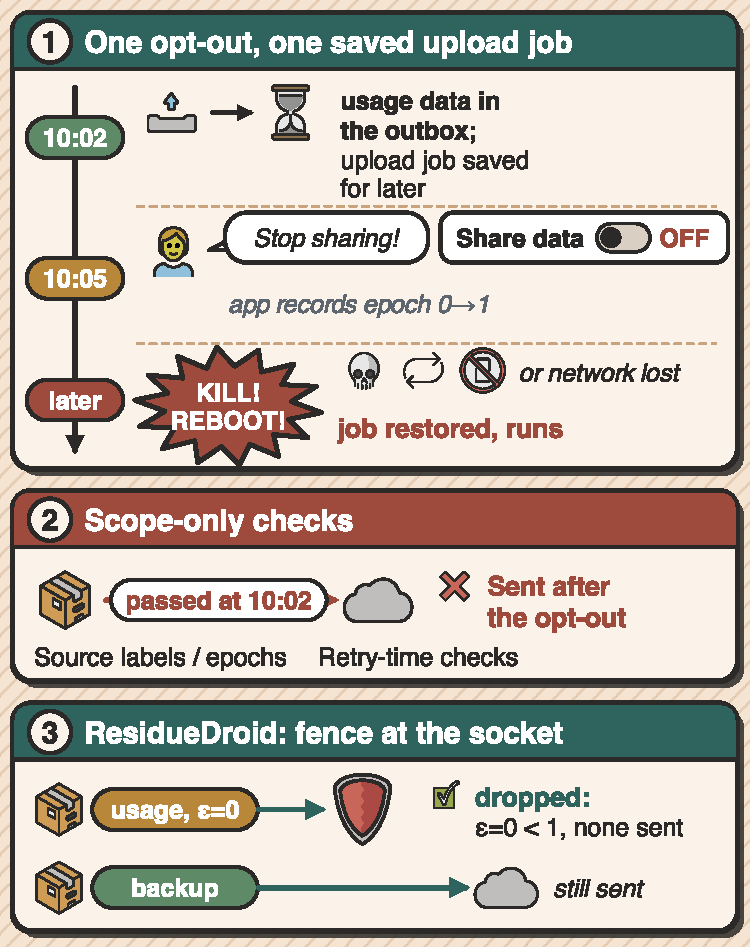
\includegraphics[width=\columnwidth]{figures/fig1.pdf}
\caption{(1)~A saved upload job outlives an opt-out across a kill, a reboot or a network loss. (2)~Checks made before submission let the data through. (3)~With \sys the label travels with the data and the fence at the socket drops it, while permitted flows such as backup still go out. Panel 2 names the information and retry checks needed by the fixture; it reports no population failure rate. Bytes already accepted before the opt-out are not recalled. Icons: OpenMoji (CC BY-SA 4.0).}
\Description{Comic with a vertical timeline panel and two stacked outcome panels. At 10:02 usage events and a summary go into an outbox and an upload job is saved; at 10:05 the user turns the Share data toggle off; later the process is killed, the device reboots or the network drops and the job is restored. With checks made earlier the data is sent after the opt-out. With ResidueDroid the labelled usage data is dropped at a fence at the socket while a backup flow is still sent.}
\label{fig:overview}
\end{figure}


Mobile apps rarely send data the moment they collect it. Usage events, crash reports, location history and derived
summaries go into a local outbox. A deferred job uploads them later, when the device has connectivity, is charging, or the
batch is large enough. Android makes this deferral durable on purpose. \texttt{JobScheduler} restores persisted jobs after
reboot, WorkManager keeps its own database of pending work~\cite{android_jobscheduler,android_workmanager}, and analytics SDKs
flush their outboxes when the app starts. Durability is what makes background uploads reliable. It also means that the upload
path can outlive the user's decision to stop it.

Consider an app whose settings say ``Share usage data''. It has queued twelve events and a summary derived from them when the user
switches the toggle off (Figure~\ref{fig:overview}). The app does the usual things. It stops collecting, it may cancel the
upload job, and its job checks the toggle before it starts. But the summary was copied into a job filed under
``diagnostics''. The process is killed and the job is restored by the system. Or the network drops after the job has started
and its retry loop resends the batch it already prepared. In each case data that the app promised to stop sending leaves the
device after the promise was made. The integration lacks a check that remains effective until socket handoff.

This paper is about that gap, and it is deliberately narrow. Withdrawal inconsistency itself is not new.
MowChecker~\cite{du2024mowchecker} statically finds withdrawal choices that do not control third-party collection.
CleanOS~\cite{tang2012cleanos}, Pebbles~\cite{spahn2014pebbles} and Weir~\cite{nadkarni2016weir} established data management
and information-flow enforcement on Android. Taint tracking~\cite{enck2010taintdroid,arzt2014flowdroid} finds flows to the
network. Two problems remain. The first is \emph{deferred} egress: data collected before an explicit withdrawal reaches the
network afterwards through persisted work, across process death, reboot and connectivity changes. The second is where a
cooperative app must enforce its own contract so that no lifecycle interleaving defeats it. We also refuse two simplifications.
First, a stored residue is not a violation. An OS permission revocation, an in-app opt-out, a processing restriction and a
deletion request are different contracts (\S\ref{sec:contracts}), and we judge each workload against the one it states.
Second, bytes already handed to the network cannot be recalled. A device-side mechanism can only control what it
\emph{newly} commits.

\paragraph{Approach.} \sys combines three small mechanisms. Durable per-scope \emph{epochs} turn a withdrawal into a
transaction. \emph{Persistent job lineage} stores a label of source scopes and epochs in the same row, or the same
persisted job input, as every copy of the data, including derived data. A \emph{late egress fence} evaluates the app's stated
contract before each bounded nonblocking socket write, inside a critical section shared with withdrawal. Under complete
mediation, durable labels and this serialization, no newly accepted supported prefix carries a source that the current policy invalidates (Theorem~\ref{thm:sound}). An earlier check without effective later cancellation admits a violating interleaving when withdrawal invalidates the source; its
probability follows from the job's commit timing (Theorem~\ref{thm:race}).

\paragraph{Evidence.} The evaluation separates information requirements from final placement.
The \corpusN-app static screen identifies candidate deferred paths, without inferring violations (\S\ref{sec:measure}).
The ten-tenant fixture exposes source-lineage loss in derived summaries (T1), stale epochs after re-grant (T5), and unchecked retry paths (T8).
These are mechanism-specific counterexamples whose frequencies depend on the selected workload mix (\S\ref{sec:eval}).
When layered early checks receive the same durable metadata, they have no confirmed violations in the measured lifecycle schedules; the fence's additional benefit is confined to a residual check-to-write interleaving, demonstrated separately with a controlled HTTPS buffering barrier.
The ACRA preference-only embedding uploads a queued report in \acraStockLeak{} trials after the harness disables reporting. It has no user-facing promise to delete that queue, so this observation alone is not a contract violation. A separate setting explicitly invalidates queued reports and exercises the fenced integration (\S\ref{sec:eval-acra}).

\paragraph{Contributions.}
(1) A contract-separated formulation of deferred egress after withdrawal, with an oracle that judges each submission
against the stated contract at an explicitly stated observation boundary. (2) \sys's persistent job lineage and serialized late fence, with a
soundness theorem for supported paths, a race theorem for earlier check points, and information requirements for lineage and
epochs. (3) A static measurement of an F-Droid corpus, a real-library case study, and a controlled emulator evaluation with
permitted-flow controls, matched transports and explicit uncovered paths. The artifact includes sources, raw logs, exclusions and deterministic generators.
